%\part{Cayley-Graphen und Automorphismengruppen}

% =============
\section{Cayley-Graphen von Gruppen}\label{sec_cayley}

\BEM\
\begin{enumerate}
\item Für jeden Graphen $\GR$ bildet die Menge $\Aut(\GR)$ der
Automorphismen von $\GR$ eine Gruppe.\index{Automorphismengruppe}\index{Gruppe!Automorphismen}
\item $\Aut(\GR)$ ist eine Untergruppe von
$\perm(E(\GR)) \times \perm(K(\GR))$.
\item Ist $\GR$ ein kombinatorischer Graph, so ist
$\Aut(\GR)\leq \perm(E(\GR))$.
\end{enumerate}

\BSP\
\begin{enumerate}
\item Für
\begin{center}
%	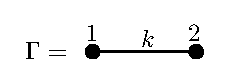
\includegraphics{aut1}
\end{center}
ist $\Aut(\GR)=\{\id,\sigma\}\cong \ZZ/2\ZZ$ mit
$\sigma(1)=2$, $\sigma(2)=1$ und $\sigma(k)=\bar{k}$.
\item Für
\begin{center}
%	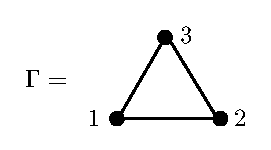
\includegraphics{aut2}
\end{center}
besteht $\Aut(\GR)$ aus sechs Elementen, es muss also
$\Aut(\GR)\cong \sym_3$ sein.
\item Für
\begin{center}
%	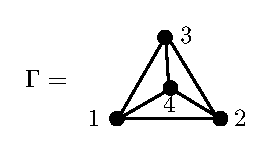
\includegraphics{aut3}
\end{center}
ist $\Aut(\GR)\cong \sym_4$.
\item Die Automorphismengruppe von
\begin{center}
%	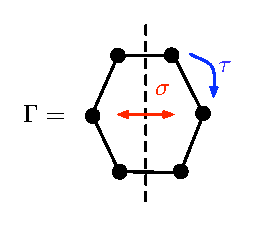
\includegraphics{aut4}
\end{center}
enthält sechs Drehungen drei Spiegelungen mit Spiegelachse
durch zwei Ecken und drei Spiegelungen mit Spiegelachse durch
Kantemittelpunkte, hat also mindestens zwölf Elemente.
In der Tat ist bereits
\[
\Aut(\GR) = \{\id,\tau,\ldots,\tau^5,
	\sigma,\sigma\tau,\ldots,\sigma \tau^5 \}
\cong \mathrm{D}_6.
\]
$\mathrm{D}_6$ ist die Diedergruppe des Sechsecks.
\end{enumerate}

\DB Es sei $G$ eine Gruppe und $S\subset G$.
Der \emph{Cayley-Graph}\index{Cayley-Graph}\index{Graph!Cayley-}\index{Gruppe!Cayley-Graph}
$\GR(G,S)$ von $G$ bzgl. $S$ wird wie folgt definiert:
\begin{align*}
E(\GR(G,S)) &:= G, \\
K(\GR(G,S)) &:= G \times S \times \{-1,1\},
\end{align*}
und für $k=(g,s,\eps)\in K(\GR(G,S))$ sei $\bar{k}=(g,s,-\eps)$
und
\begin{align*}
&\ini(k) = g, \quad \ter(k) = gs \quad \text{falls } \eps = 1, \\
&\ini(k) = gs, \quad \ter(k) = g \quad \text{falls } \eps = -1.
\end{align*}

\BSP\label{bsp_cay}\
\begin{enumerate}
\item Es sei $G$ beliebig, $S=\emptyset$.
Dann ist $K(\GR(G,S))=\emptyset$.
\item $G=\ZZ$ und $S=\{1\}$:
\begin{center}
%	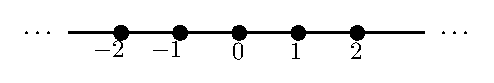
\includegraphics{cay1}
\end{center}
\item $G=\ZZ$ und $S=\{2\}$:
\begin{center}
%	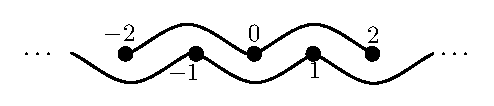
\includegraphics{cay3}
\end{center}
\item $G=\ZZ$ und $S=\{-1,1\}$:
\begin{center}
%	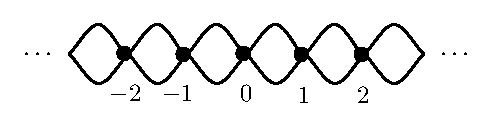
\includegraphics{cay2}
\end{center}
\item $G=\ZZ/n\ZZ$ und $S=\{1\}$:
\begin{center}
%	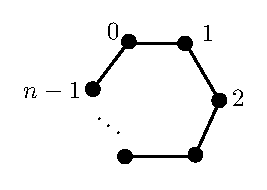
\includegraphics{cay4}
\end{center}
\item $G=\sym_3$ und $S=\{\tau=(1\ 2\ 3),\sigma=(1\ 2)\}$.
Es ist $\sym_3=\{\id,\tau,\tau^2,\sigma,\sigma\tau,\sigma\tau^2\}$.
\begin{center}
%	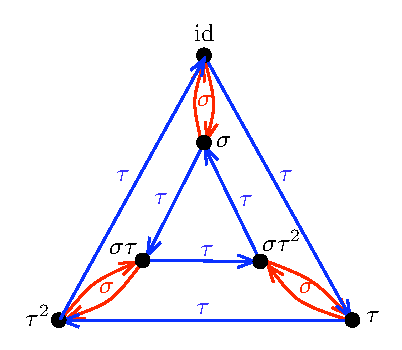
\includegraphics{cay5}
\end{center}
Man beachte, dass für die Kantenübergänge von rechts multipliziert 
wird.
\end{enumerate}

\BEM\label{bem_GRGS}\
\begin{enumerate}
\item $\GR(G,S)$ ist genau dann zusammenhängend, wenn
$G$ von der Menge $S$ erzeugt wird.
\item Für jede Ecke $g\in G=E(\GR(G,S))$ ist $v(g)=\frac{1}{2}|S|$.
\item $\GR(G,S)$ enthält genau dann Schleifen, wenn $1$ in $S$
enthalten ist.
\item $\GR(G,S)$ enthält genau dann Doppelkanten, wenn es in $S$
Elemente $s\neq 1$ gibt, so dass auch $s^{-1}\in S$ ist.
\item $\GR(G,S)$ enthält keine Dreifachkanten.
\end{enumerate}
\textsc{Beweis von 1.:} \glqq$\ra$\grqq: Sei $g\in G$ beliebig und
$w=(k_1,\ldots,k_n)$ ein Weg in $\GR(G,S)$ von $1$ nach $g$,
mit $k_i=(g_i, s_i, \eps_i)$. Dann ist
$g_1=1$, $g_2=s_1^{\eps_1}$, \ldots,
$g_n=s_1^{\eps_1}\cdots s_{n-1}^{\eps_{n-1}}$.
Somit ist $g=\ter(k_n)=g_n s_n^{\eps_n}=
s_1^{\eps_1}\cdots s_n^{\eps_n} \in\lag S\rag$.\\
\glqq $\la$\grqq: Führe die gleiche Überlegung rückwärts durch.
\qed

\DB Es sei $G$ eine Gruppe und $\GR$ ein beliebiger Graph.
\begin{enumerate}
\item Eine \emph{Aktion}\index{Aktion}\index{Gruppe!Aktion} (oder \emph{Operation}\index{Operation (siehe Aktion)}) von $G$ auf $\GR$ ist ein
Gruppenhomomorphismus $\rho:G\Ra\GR$.
\item Eine Aktion heißt \emph{treu}\index{Aktion!treu}\index{treue Aktion}
(oder \emph{effektiv}\index{effektiv (siehe treue Aktion)}\index{Aktion!effektiv}),
wenn $\K{\rho}=\{1\}$ ist. Der Kern von $\rho$ heißt auch
\emph{Ineffektivitätskern}\index{Ineffektivitätskern}
der Aktion $\rho$.
\end{enumerate}

\BEM Es sei $G$ eine Gruppe, $S\subset G$. Dann operiert $G$ von
links auf $\GR(G,S)$ und diese Operation ist treu.\\
Genauer: Für $g\in G$ sei $\phi_g:\GR(G,S)\Ra\GR(G,S)$ gegeben durch
\begin{align*}
\phi_g(g') &= gg', \\
\phi_g(g',s,\eps) &= (gg',s,\eps).
\end{align*}
Dann gilt:
\begin{enumerate}
\item $\phi_g \in \Aut(\GR(G,S))$.
\item $\phi:G\Ra\Aut(\GR(G,S)), g\mapsto \phi_g$ ist ein injektiver
Gruppenhomomorphismus.
\end{enumerate}

\BSP (vgl. Beispiel \ref{bsp_cay})
\begin{enumerate}
\item $\ZZ$ operiert auf $\GR(Z,\{1\})$ durch Translation.
\item $\ZZ/n\ZZ$ operiert auf $\GR(\ZZ/n\ZZ,\{1\})$ durch
Drehungen. Hier ist $\phi:G\Ra\Aut(\GR(G,S))$, $g\mapsto\phi_g$
injektiv, aber nicht surjektiv (da Spiegelungen nicht durch
$\phi$ dargestellt werden).
\item $G=\sym_3$ und $S=\{\tau=(1\ 2\ 3), \sigma=(1\ 2)\}$.
\begin{center}
%	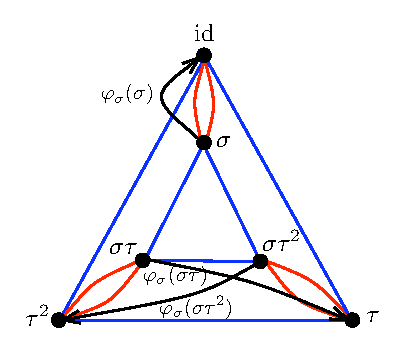
\includegraphics{S3aktion}
\end{center}
$\phi_{\tau}$ ist die Drehung um $120^{\circ}$ im
Uhrzeigersinn. $\phi_{\sigma}$ vertauscht rechts mit links und
innen mit außen.
\end{enumerate}

\PROP Es sei $G$ eine Gruppe, $S\subset G$, und $G_S=\lag S\rag$
bezeichne die von $S$ erzeugte Untergruppe.
\begin{enumerate}
\item Die Zusammenhangskomponenten von $\GR(G,S)$ entsprechen
bijektiv den Linksnebenklassen $g G_S$ für $g\in G$.
\item Es sei $S'\subseteq S$ und $H:=\lag S'\rag \leq G_S$.
Sei $\GR_H(G,S)$ der Graph, der aus $\GR(G,S)$ durch Kontraktion
von $\GR(G,S')$ entsteht.
Dann operiert $G$ auf $\GR_H(G,S)$.
Es ist $E(\GR_H(G,S)) = G/H$ (die Menge der Nebenklassen).
\end{enumerate}
\bew \begin{enumerate}
\item Es bezeichne $\GR_g$ diejenige Zusammenhangskomponente von
$\GR$, die die Ecke $g\in G$ enthält.\\
Die Zusammenhangskomponente $\GR_1$ von $\GR(G,S)$ ist isomorph
zu $\GR(G_S,S)$ (vgl. Bemerkung \ref{bem_GRGS}(1)).
Betrachte $\GR_g$ für beliebiges $g\in G$. Es ist $\phi_g(1)=g$,
also hat $\phi_g(\GR_1)$ nichtleeren Schnitt mit $\GR_g$ und ist
zusammenhängend. Es folgt $\phi_g(\GR_1)=\GR_g$.
Somit ist
\[
E(\GR_g)=(\phi_g)_E(E(\GR_1))=(\phi_g)_E(G_S) = g G_S.
\]
\item
Es ist $K(\GR_G(G,S))=G\times S-S'\times\{-1,1\}$ mit
$\ini(g,s,1)=gH$, $\ter(g,s,1)=gsH$.
Ein Element $g\in G$ operiert wie folgt:
\begin{align*}
g(g'H) &= (gg')H, \\
g(g',s,\eps) &= (gg',s,\eps).
\end{align*}
Aus Teil 1 folgt $E(\GR_H(G,S))=G/H$.
\qed
\end{enumerate}

Wir betrachten nun den Graphen, der aus $\GR$ durch Zusammenfassen
aller Mehrfachkanten und Weglassen von Schleifen entsteht
(wobei die Orientierung jedoch beibehalten wird).

\BEM Sei $\GR$ ein Graph und $\bar{\GR}$ mit
\begin{gather*}
E(\bar{\GR}) = E(\GR), \\
K(\bar{\GR}) =
\{(x,y)\in E(\GR)\times E(\GR) : \exists k\in
	K(\GR)\backslash\{\text{Schleifen}\}:
	\ini(k)=x, \ter(k)=y \},
\end{gather*}
mit $\bar{(x,y)}:=(y,x)$, $\ini(x,y):=x$ und $\ter(x,y):=y$.
\begin{enumerate}
\item Die Abbildung $p:\GR\Ra\bar{\GR}$, $p_E=\id$,
$p_K(k)=(\ini(k),\ter(k))$ ist ein surjektiver Morphismus von
Graphen.
\item Es gibt einen eindeutig bestimmten Gruppenhomomorphismus
$\rho:\Aut(\GR)\Ra\Aut(\bar{\GR})$, so dass für alle
$\gamma\in\Aut(\GR)$ das folgende Diagramm kommutiert:
\[\xymatrix{
\GR \ar[r]^{\gamma} \ar[d]_{p} & \GR \ar[d]^{p} \\
\bar{\GR} \ar[r]_{\rho(\gamma)} & \bar{\GR}
}\]
\item
Es ist
\[
\K{\rho} = \{ \gamma\in\Aut(\GR) : \gamma_E=\id \}.
\]
\end{enumerate}
\textsc{Beweis von 2.:} Definiere $\bar{\gamma}\in\Aut(\bar{\GR})$
durch $\bar{\gamma}_E := \gamma_E$ und
$\bar{\gamma}_K(x,y) := (\ini(\gamma(k)),\ter(\gamma(k)))$
für $(x,y)\in K(\bar{\GR})$, $k\in K(\GR)$ mit $p_K(k)=(x,y)$.
Setze nun $\rho(\gamma):=\bar{\gamma}$.
\qed

\FOLG Es sei $G$ eine Gruppe und $\GR$ ein beliebiger Graph.
\begin{enumerate}
\item Jede Aktion von $G$ auf $\GR$ induziert eine Aktion auf
$\bar{\GR}$.
\item Ist $\GR=\GR(G,S)$ ein Cayley-Graph, so operiert $G$ treu
auf $\GR$ und $\bar{\GR}$.
\item Ist $\GR=\GR_H(G,S)$, so ist die Aktion $\rho$ von $G$ auf
$\bar{\GR}$ genau dann treu, wenn gilt
\[
\BCAP{}{g\in G} gHg^{-1} = \{1\}.
\]
\end{enumerate}
\textsc{Beweis von 3.:} \glqq$\ra$\grqq:
Die Ecken von $\GR$ sind die Linksnebenklassen
$gH$, $g\in G$. Sei $h\in G$ mit $\rho(g)=\id$. Dann ist
$hgH=gH$ für alle $g\in G$, d.h. $g^{-1}hg=h'\in H$.
Folglich ist $h=gh'g^{-1}\in gHg^{-1}$, und da dies für alle
$g\in G$ gilt, ist $h\in \bigcap_{g\in G} gHg^{-1}$.\\
\glqq$\la$\grqq: Ist $h\in \bigcap_{g\in G} gHg^{-1}$, so ist
$\rho(h)_E=\id_{E(\GR)}=\id_{E(\bar{\GR})}$.
Somit ist $\rho(h)=\id$.
\qed

\SATZ\label{satz_abzb} Es sei $G$ eine abzählbare Gruppe. Dann gibt es einen
zusammenhängenden Graphen $\GR$ mit $\Aut(\GR)\cong G$.

Das folgende Beispiel soll die Idee des anschließenden Beweises
veranschaulichen.
\BSP Betrachte die Kleinsche Vierergruppe\index{Kleinsche Vierergruppe}
$G=\mathrm{V}_4(=\mathrm{D}_2)=\{1,\sigma,\tau,\sigma\tau\}$
mit $S=\{\sigma,\tau\}$.
Es ist
\begin{center}
%	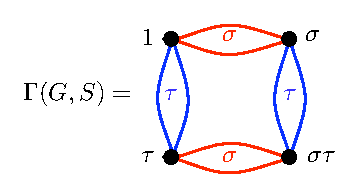
\includegraphics{klein41}
\end{center}
Die Automorphismengruppe dieses Graphen ist aber größer als
$\mathrm{V}_4$. Die Idee ist nun, die $\tau$- bzw. $\sigma$-Kanten
durch \glqq Markierungen\grqq unterscheidbar zu machen,
so dass sie nichtmehr ausgetauscht werden können:
\begin{center}
%	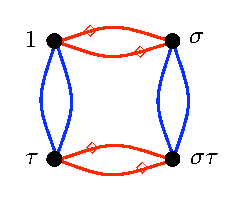
\includegraphics{klein42}
\end{center}
Durch weitere Markierungen wird verhindert, dass Kanten mit ihren
Gegenkanten vertauscht werden:
\begin{center}
%	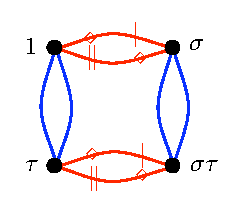
\includegraphics{klein43}
\end{center}

\textsc{Beweis von Satz \ref{satz_abzb}:}
Es sei $S=\{s_1, s_2, \ldots\}$ ein abzählbares Erzeugendensystem
und $\GR_0=\GR(G,S)$.
Für $i\geq 1$ sei $T_i$ der Baum
\begin{center}
%	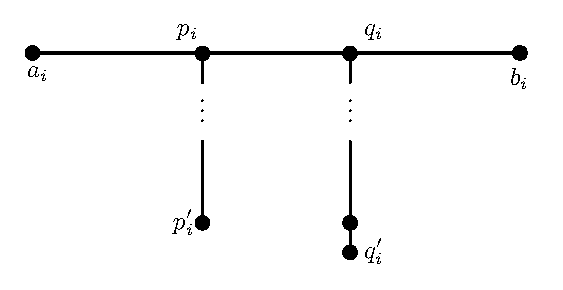
\includegraphics{Ti}
\end{center}
mit $d(p_i,p_i')=2i$ und $d(q_i,q_i')=2i+1$.
Dann ist $T_i\not\cong T_j$ für $i\neq j$ und $\Aut(T_i)=\{\id\}$
für alle $i$. Sei $\GR$ der Graph, der aus $\GR_0$ entsteht, indem
jeder Teilbaum
\begin{center}
%	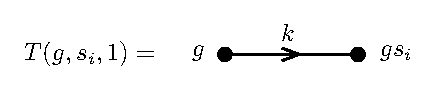
\includegraphics{ggsi}
\end{center}
mit $k=(g,s_i,1)$ durch den Baum $T_i$ ersetzt wird.
Die Abbildung
\[
\GR\Ra\GR_0,\quad T_i\mapsto T(g,s_i,1)
\]
ist ein surjektiver Morphismus.
Nun operiert $G$ auf $\GR$ und jeder Automorphismus von $\GR$
induziert einen Automorphismus von $\GR_0$, der \glqq farbtreu\grqq\
ist.

Ist $\gamma\in\Aut(\GR)$ und $x\in E(\GR)$ mit $\gamma_E(x)=x$,
so ist $\gamma=\id$, denn für $x\not\in E(\GR_0)$ gibt es $i\geq 1$
mit $x\in E(T_i)\backslash\{a_i,b_i\}$.
Dann ist $\gamma|_{T_i}=\id_{T_i}$ und somit ohne Einschränkung
$x\in E(\GR_0)$. Es gibt für jedes $s_i\in S$ genau eine Kante der
Form $(x,s_i,1)$ in $\GR_0$, also in $\GR$ genau einen Baum $T_i$
mit $a_i=x$. Also ist $\gamma=\id$ auf jedem dieser Teilbäume.
Mit Induktion bzw. Anwendung des Zornschen Lemmas folgt, dass
$\gamma$ die Identität ist.

Nun zeigen wir $\Aut(\GR)=G$: Dazu sei $\gamma\in\Aut(\GR)$ und
$g\in E(\GR_0)=G$. Es sei $g':=\gamma_E(g)\in E(\GR_0)=G$
und $h=g'g^{-1}\in G$. Dann ist $\rho(h)_E(g)=hg=g'$.
Es folgt $(\gamma^{-1}\circ\rho(h))_E(g)=g$, also
ist nach dem eben Gezeigten $\gamma^{-1}\circ\rho(h)=\id$ und somit
$\gamma=\rho(h)$.
\qed

% ====================
\section{Quotientengraphen}\label{sec_qg}

\DEF Es sei $\rho:G\Ra\Aut(\GR)$ eine Aktion der Gruppe $G$ auf einem
Graphen $\GR$. Wenn für alle $g\in G$ und alle $h\in K(\GR)$ gilt
\[
\rho(g)_K(k) \neq \bar{k},
\]
so heißt $\rho$ \emph{inversionsfrei}\index{inversionsfreie Aktion}\index{Aktion!inversionsfrei}.

\DB Es sei $\rho:G\Ra\Aut(\GR)$ eine inversionsfreie Aktion.
Dann gibt es einen eindeutig bestimmten
\emph{Quotientengraphen}\index{Quotientengraph}\index{Graph!Quotienten-}
$\GR/G$ mit
\begin{align*}
E(\GR/G) &= E(\GR)/G \quad\text{(Menge der Bahnen)},\\
K(\GR/G) &= K(\GR)/G.
\end{align*}
Weiter gelten:
\begin{enumerate}
\item Für $Gk:=\rho(G)_K(k)$ ist $\bar{Gk}=G\bar{k}$.
\item Es ist $\ini(Gk)=G \ini(k)$ und $\ter(Gk)=G\ter(k)$.
\item Die kanonische Projektion
	$p:\GR\Ra\GR/G$ ist ein surjektiver Morphismus von Graphen.
\item Ist $f:\GR\Ra\GR'$ ein $G$-invarianter Morphismus von
Graphen (d.h. es ist $f\circ\rho(g)=f$ für alle $g\in G$),
so gibt es genau einen Morphismus
$\bar{f}:\GR/G\Ra \GR'$ mit $f=\bar{f}\circ p$.
\[\xymatrix{
\GR \ar[r]^{f} \ar[d]_{p} & \GR' \\
\GR/G \ar[ru]_{\bar{f}} &
}\]
\end{enumerate}

\BSP\
\begin{enumerate}
\item Für $\GR=\GR(\ZZ,\{1\})$ operiert $G=\ZZ$ durch
Translation. Es ist
\begin{center}
%	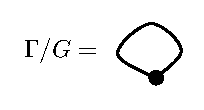
\includegraphics{quot1}
\end{center}
\item Für eine beliebige Gruppe $G$ operiert $G$ auf
$\GR=\GR(G,S)$ durch Linksmultiplikation.
Somit ist
\begin{center}
%	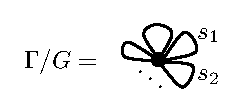
\includegraphics{quot2}
\end{center}
wobei die Anzahl der Schleifen gleich $|S|$ ist.
\item Es sei
\begin{center}
%	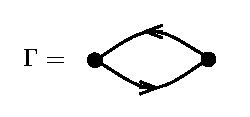
\includegraphics{quot3}
\end{center}
Dann operiert $G=\ZZ/2\ZZ$ auf $\GR$ durch
\begin{itemize}
\item Spiegelung an der horizontalen Achse:
\begin{center}
%	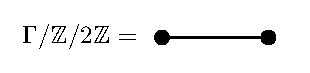
\includegraphics{quot3a}
\end{center}
\item Spiegelung an der vertikalen Achse; in diesem Fall ist
die Operation nicht inversionsfrei.
\item
Drehung um $180^\circ$:
\begin{center}
%	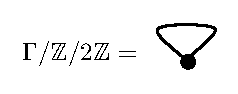
\includegraphics{quot3b}
\end{center}
\end{itemize}
\end{enumerate}

\BEM Sei $\GR$ ein zusammenhängender Graph und $\rho:G\Ra\Aut(\GR)$
eine inversionsfreie Aktion.
Dann lässt sich jeder Teilbaum von $\GR/G$ nach $\GR$ liften,
d.h. zu einem Teilbaum $T'$ in $\GR/G$ gibt es einen Teilbaum $T$ in
$\GR$, so dass $p|_T:T\Ra T'$ ein Isomorphismus ist.

\bew Es sei
$\calT =\{ T \subset \GR : p|_T \text{ ist injektiv und } p(T)\subseteq T' \}$.
Sofern $\GR\neq\emptyset$, ist auch $\calT\neq\emptyset$.
Außerdem ist $\calT$ durch die Inklusionsrelation partiell geordnet.
Nach dem Zornschen Lemma enthält $\calT$ also ein maximales Element
$T_0$.

Zu zeigen ist nun, dass $p(T_0)=T'$ ist.
Wäre dies nicht der Fall, so können wir in $T'$ eine erste Kante
wählen, die nicht mehr in $p(T_0)$ liegt, genauer gesagt gibt es eine
Kante $k'\in K(T')$ mit $k'\not\in K(p(T_0))$ und
$\ini(k')\in E(p(T_0))$. Dann muss $\ter(k')\not\in E(p(T_0))$ gelten,
denn $p(T_0)$ ist ein Baum, also insbesondere zusammenhängend.
Falls also $\ter(k')\in p(T_0)$ wäre, so gäbe es einen stachelfreien
Weg $w$ in $p(T_0)$ von $\ini(k')$ nach $\ter(k')$.
Dann wäre $(w, \bar{k}')$ ein Kreis in $T'$, im Widerspruch dazu,
dass $T'$ ein Baum ist.\\
Nun sei $\tilde{k}\in p^{-1}(k')$, also
$p(\ini(\tilde{k}))=\ini(k') \in E(p(T_0))$.
Sei $x_0 \in E(T_0)$ die eindeutige Ecke mit $p_E(x_0)=\ini(k')$.
Dann muss es ein $g\in G$ geben mit $g(\ini(\tilde{k}))=x_0$.
Für $k:=g(\tilde{k})$ gilt dann $\ini(k)=x_0$ und $p(k)=k'$.
Somit gilt $k\not\in K(T_0)$ und $\ter(k)\not\in E(T_0)$.
Indem man zu $T_0$ die Kanten $k,\bar{k}$ und die Ecke $\ter(k)$
hinzunimmt, erhält man einen Teilbaum in $\calT$, der $T_0$ als
echten Teilbaum enthält, im Widerspruch zur Maximalität von $T_0$.
Also muss $p(T_0)=T'$ sein.
\qed

\BSP $G=\ZZ/2\ZZ$ operiert auf $\GR$.
\begin{center}
%	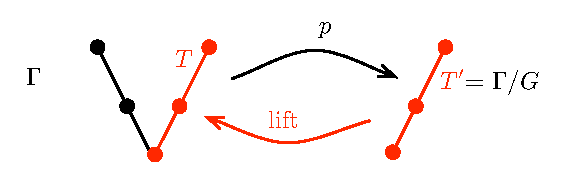
\includegraphics{lift}
\end{center}

Wir betrachten nun den Graphen, der entsteht, indem man jede Kante $k$
eines Graphen $\GR$ durch Einfügen einer weiteren
Ecke unterteilt. Diese neue Ecke kann formal mit der geometrischen
Kante $[k]=\{k,\bar{k}\}$ identifiziert werden.

\DEF Es sei $\GR$ ein Graph. Der Graph $\GRsub$ mit
\begin{align*}
E(\GRsub) &= E(\GR)\cup\{\text{geometrische Kanten von }\GR\} \\
K(\GRsub) &= K(\GR)\times\{-1,1\}
\end{align*}
und
$\ini(k,1)=\ini(k)$, $\ter(k,1)=\ini(k,-1)=[k]$,
$\ter(k,-1)=\ter(k)$ und $\bar{(k, \pm 1)}=(\bar{k},\mp 1)$
heißt \emph{baryzentrische Unterteilung}\index{baryzentrische Unterteilung}\index{Unterteilung}\index{Graph!Unterteilung}\index{Graph!baryzentrische Unterteilung}
von $\GR$.
\begin{center}
%	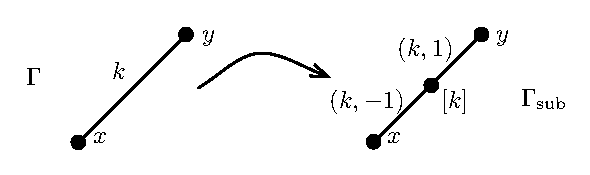
\includegraphics{subdiv}
\end{center}

\BEM Sei $\GR$ ein Graph.
\begin{enumerate}
\item $\GRsub$ hat keine Schleifen.
\item $\GRsub$ ist genau dann zusammenhängend, wenn $\GR$
	zusammenhängend ist.
\item $\GRsub$ ist genau dann ein Baum, wenn $\GR$ ein Baum ist.
\item Ist $\GR$ zusammenhängend, so ist $g(\GR)=g(\GRsub)$.
\end{enumerate}

\BEM Jede Aktion $\rho:G\Ra\Aut(\GR)$ induziert eine inversionsfreie
Aktion $\rhosub:G\Ra\Aut(\GRsub)$.

\bew Definiere $\rhosub$ durch
\[
\rhosub(g)_E(x) :=
\left\{\begin{matrix}
\rho(g)_E(x), & x\in E(\GR) \\
[\rho(g)_K(k)], & x=[k]
\end{matrix}\right.
\]
und
\[
\rhosub(g)_K(k,\eps) :=
(\rho(g)_K(k),\eps),
\quad \eps=\pm 1.
\]
Die Inversionsfreiheit folgt daraus, dass das Vorzeichen von $\eps$
bei der Aktion von $\rho(g)$ erhalten bleibt.
\qed

% =====================
\section{Freie Gruppen}\label{sec_FG}

Definition und erste Eigenschaften einer freien Gruppe $F(X)$
mit Erzeugermenge $X$ findet man in Kapitel I.12 von Lang \cite{lang}.
\index{freie Gruppe}\index{Gruppe!frei}
Wir davon werden wir insbesondere die folgenden benötigen:
\begin{itemize}
\item Für $|X|\geq 2$ ist $F(X)$ nicht abelsch.
\item $F(X)\cong F(Y)$ genau dann, wenn $|X|=|Y|$.
\item Die \emph{universelle Abbildungseigenschaft (UAE)}\index{universelle Abbildungseigenschaft}\index{UAE}
der freien Gruppen besagt, dass es für eine beliebige Gruppe $G$ und
eine Abbildung $f:X\Ra G$ einen eindeutigen Gruppenhomomorphismus
$\phi:F(X)\Ra G$ gibt mit $\phi(x)=f(x)$ für alle $x\in X$.
\end{itemize}

\PROP Es sei $G$ eine Gruppe und $S\subseteq G$. Dann gilt
$G\cong F(S)$ genau dann, wenn $\GR(G,S)$ ein Baum ist.

\bew \glqq$\ra$\grqq:
$\GR(G,S)$ ist zusammenhängend, da $\lag S\rag=G$. Es bleibt zu
zeigen, dass keine Kreise der Länge $\geq 1$ existieren.\\
Es sei $w=(k_1,\ldots,k_n)$ ein Kreis in $\GR(F(S),S)$ mit
$k_i=(g_i,s_i,\eps_i)$.
Es ist $\ter(w)=g_1 s_1^{\eps_1}\cdots s_n^{\eps_n}
=\ini(w)=g_1$, also $s_1^{\eps_1}\cdots s_n^{\eps_n}=1$.
Da $w$ stachelfrei ist, ist $s_1^{\eps_1}\cdots s_n^{\eps_n}$
reduziert und es folgt $n=0$.\\
\glqq$\la$\grqq:
$S$ erzeugt $G$, da $\GR(G,S)$ zusammenhängend ist.
$S\cap S^{-1}=\emptyset$, da keine Doppelkanten und Schleifen
in $\GR(G,S)$ vorkommen. Wir erhalten einen Gruppenhomomorphismus
$\phi:F(S)\Ra G$ durch $s\mapsto s$.
Dieses $\phi$ ist surjektiv, da $S$ eine Erzeugermenge ist.
Angenommen, $\phi$ sei nicht injektiv. Dann gibt es ein
$s_1^{l_1}\cdots s_n^{l_n} \in \K{\phi}$ mit $n>0$ minimal.
Dann sind $1,s_1^{l_1},\ldots,s_1^{l_1}\cdots s_{n-1}^{l_{n-1}}$
Ecken eines geschlossenen Weges in $\GR(G,S)$, im Widerspruch dazu,
dass $\GR(G,S)$ ein Baum ist. Somit muss $\K{\phi}=\{1\}$ sein
und $\phi$ ist injektiv.
\qed

\BSP Der Cayley-Graph der freien Gruppe mit zwei Erzeugern
$F_2=F(\{x,y\})$.
\begin{center}
%	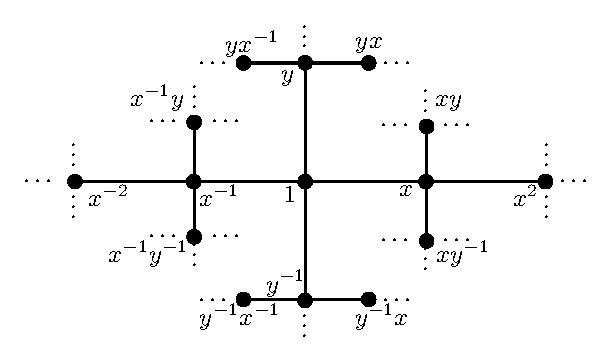
\includegraphics{Fxy}
\end{center}